%%%%%%%%%%%%%%%%%%%%%%%%%%%%%%%%%%%%%%%%%%%%%%%%%%%%%%%%%%%%
%%  This Beamer template was created by Cameron Bracken.
%%  Anyone can freely use or modify it for any purpose
%%  without attribution.
%%
%%  The current presentation created by Jeferson L. R. Souza (jefecomp) is based on the template created by Cameron Bracken. 
%%  
%%  Small modifications have been introduced and anyone is free to use such modified version.
%%
%% Last Modified: June 14, 2015.

\documentclass[xcolor=x11names,compress]{beamer}

%% General document %%%%%%%%%%%%%%%%%%%%%%%%%%%%%%%%%%
\usepackage{graphicx}
\usepackage{tikz}
\usetikzlibrary{decorations.fractals}
%%%%%%%%%%%%%%%%%%%%%%%%%%%%%%%%%%%%%%%%%%%%%%%%%%%%%%

%Hyperref
\usepackage{hyperref}

%Multirow package
\usepackage{multirow} 

%Math packages
\usepackage{amsmath}
\usepackage{textcomp}


%% Beamer Layout %%%%%%%%%%%%%%%%%%%%%%%%%%%%%%%%%%
\useoutertheme[footline=authorinstitutetitle,subsection=false,shadow]{miniframes}
\useinnertheme{default}
\usefonttheme{professionalfonts}
\usepackage{mathpazo}

\setbeamerfont{title like}{shape=\scshape,series=\bfseries}
\setbeamerfont{frametitle}{shape=\scshape,series=\bfseries}

\setbeamercolor*{lower separation line head}{bg=Green3} 
\setbeamercolor*{upper separation line foot}{bg=Green3} 
\setbeamercolor*{normal text}{fg=black,bg=white} 
\setbeamercolor*{alerted text}{fg=black,bg=black!10} 
\setbeamercolor*{example text}{fg=black} 
\setbeamercolor*{structure}{fg=black}
 
\setbeamercolor*{palette tertiary}{fg=black,bg=black!3} 
\setbeamercolor*{palette quaternary}{fg=black,bg=black!10} 

%%%%%%%%%%%%%%%%%%%%%%%%%%%%%%%%%%%%%%%%%%%%%%%%%%

\setbeamertemplate{blocks}[rounded] [shadow=true]
\setbeamertemplate{frametitle continuation}[from second][(Continuação)]

%%  declaring picture extensions and default path
\DeclareGraphicsExtensions{.png, .jpg, .pdf}
\graphicspath{{pictures/}}

%% Supporting source code lists
\usepackage{listings}
\lstset{breakatwhitespace,
language=Java,
columns=fullflexible,
keepspaces,
breaklines,
tabsize=3, 
showstringspaces=false,
extendedchars=true}

%Text position
\usepackage{textpos}
\setlength{\TPHorizModule}{128mm}
\setlength{\TPVertModule}{96mm}

\usepackage{array}

%Puting text and other float elements over pictures
\usepackage[percent]{overpic}


%% Hyperlinks over all the document
\usepackage{hyperref}

%% Controlling text alignment
\usepackage{ragged2e}

%% Framed text
\usepackage{framed}

%% Math packages
\usepackage{amsmath}

\begin{document}

\title[Linguagem de Definição de Dados (DDL) \hskip20mm \insertframenumber / \inserttotalframenumber  \hskip33.5mm \inserttitlegraphic]{Linguagem de Definição de Dados (DDL) - Continuação \\[4mm]

\includegraphics[keepaspectratio,width=.25\textwidth]{database-server}}
\author[@2018 Prof. Jeferson Souza, MSc (jefecomp) - All rights reserved.]{
	\textcolor{blue}{Prof. Jeferson Souza, MSc.} \\[1mm] 
	\textcolor{blue}{\textit{{\footnotesize (jefecomp) }}}\\[1.5mm]
	 \underline{{\footnotesize jefecomp.official@gmail.com}}
	 \vspace*{1mm}
}
\institute[]{\centering 
\includegraphics[keepaspectratio,width=.5\textwidth]{template/logo_udesc_joinville_horizontal_assinatura}
}

\date{}

\titlegraphic{
\includegraphics[keepaspectratio,width=.2\textwidth]{template/logo_udesc_joinville_horizontal_assinatura}}

%%%%%%%%%%%%%%%%%%%%%%%%%%%%%%%%%%%%%%%%%%%%%%%%%%%%%%
%%%%%%%%%%%%%%%%%%%%%%%%%%%%%%%%%%%%%%%%%%%%%%%%%%%%%%
\begin{frame}[plain,noframenumbering]
\titlepage
\end{frame}


%%%%%%%%%%%%%%%%%%%%%%%%%%%%%%%%%%%%%%%%%%%%%%%%%%%%%%
%%%%%%%%%%%%%%%%%%%%%%%%%%%%%%%%%%%%%%%%%%%%%%%%%%%%%%
\section{Integridade}
\subsection{Restrições}
\begin{frame}{Integridade do dados}

\begin{alertblock}{Restrições de integridade}
Como visto nos slides anteriormente no material do curso é possível criar restrições na definição das tabelas do banco de dados. A definição de restrições permite especificar o modelo de consistência que os dados devem seguir, e portanto são denominadas \textbf{restrições de integridade}.
\end{alertblock}

\begin{alertblock}{Exemplos}
\begin{itemize}
\itemsep 5mm

\item O nome do usuário não pode ser nulo;

\item Dois usuários não podem ter o mesmo cpf;

\item O saldo da conta deve ser sempre maior do que R\$50,00;

\end{itemize}
\end{alertblock}

\end{frame}

\begin{frame}{Restrições de integridade}

Algumas das formas de especificar restrições de integridade já foram vistas anteriormente:

\begin{itemize}
\itemsep 5mm

\item \textbf{NULL}; 

\item \textbf{NOT NULL};

\item \textbf{UNIQUE};

\item \textbf{DEFAULT}.

\end{itemize}

Entretanto, vamos ver mais alguns exemplos da restrição \textbf{UNIQUE}.

\end{frame}

\begin{frame}{Restrições de integridade: \textit{UNIQUE}}

\begin{alertblock}{Exemplo de candidatos a chave com \textit{UNIQUE}}
\textbf{CREATE TABLE} usuario(id \textcolor{red}{serial} \textit{PRIMARY KEY}, nome \textcolor{red}{varchar}(20), email \textcolor{red}{varchar}(30), cpf \textcolor {red}{char} (11)., \textit{UNIQUE}(email,cpf));
\end{alertblock}

\end{frame}

\begin{frame}[allowframebreaks]{Restrições de integridade: \textit{CHECK}}

Com a restrição do tipo check é possível definir uma expressão (ex: preco > 0) que deve ser satisfeita durante a manipulação dos dados. 

\begin{alertblock}{Exemplo 1}
\textbf{CREATE TABLE} conta(nr\_conta \textcolor{red}{bigserial}, agencia \textcolor{red}{bigint}, saldo \textcolor{red}{numeric}, \textit{PRIMARY KEY} (nr\_conta,agencia), \textit{FOREIGN KEY}(agencia) references agencia(id), \textit{\textbf{CHECK}}(saldo > 0));
\end{alertblock}

\begin{alertblock}{Exemplo 2}
\textbf{CREATE TABLE} departamento (id \textcolor{red}{bigserial} \textit{PRIMARY KEY}, nome \textcolor{red}{varchar}(30), sigla \textcolor{red}{varchar}(4),  \textit{\textbf{CHECK}}(sigla \textbf{in} ('DCC','DMAT','DEC','DEE')));
\end{alertblock}

\begin{alertblock}{Exemplo 3}
\textbf{CREATE TABLE} departamento (id \textcolor{red}{bigserial} \textit{PRIMARY KEY}, nome \textcolor{red}{varchar}(30), sigla \textcolor{red}{varchar}(4),  \textit{\textbf{CHECK}}(sigla \textbf{in} (select sigla from siglas where tipo = 'departamento')));
\end{alertblock}

\end{frame}

\begin{frame}[allowframebreaks]{Integridade Referencial}

\begin{alertblock}{Conceito}
Integridade referencial visa garantir que um conjunto de valores que apareçam em uma determinada tabela, sejam consistentes com os valores de sua tabela de referência. 
\end{alertblock}

\begin{alertblock}{Exemplo 1}
\textbf{CREATE TABLE} usuario (id \textcolor{red}{bigserial} \textit{PRIMARY KEY}, nome \textcolor{red}{varchar}(30), dept \textcolor{red}{bigint} \textit{\textbf{references}} departamento);
\end{alertblock}

\begin{alertblock}{Exemplo 2}
\textbf{CREATE TABLE} departamento (id \textcolor{red}{bigserial} \textit{PRIMARY KEY}, nome \textcolor{red}{varchar}(30), sigla \textcolor{red}{char}(3) UNIQUE NOT NULL); \\[5mm]

\textbf{CREATE TABLE} curso (id \textcolor{red}{bigserial} \textit{PRIMARY KEY}, nome \textcolor{red}{varchar}(30), dept \textcolor{red}{char}(3) UNIQUE NOT NULL \textit{\textbf{references}} departamento (sigla));
\end{alertblock}

\begin{alertblock}{\textcolor{red}{Importante}}
Colunas que não sejam chaves primárias para serem referenciadas devem ser, pelo menos, únicas. 
\end{alertblock}

\end{frame}

\begin{frame}{Integridade Referencial: Operações em cascata}

É possível realizar operações em cascata na base de dados para manter a integridade referencial. Para isso, basta definir as chaves estrangeiras com a cláusula \textbf{cascade}. 

\begin{alertblock}{Exemplo}

\textbf{CREATE TABLE} curso (id \textcolor{red}{bigserial} \textit{PRIMARY KEY}, nome \textcolor{red}{varchar}(30), dept \textcolor{red}{char}(3) UNIQUE NOT NULL, \textit{FOREIGN KEY}(dept) \textit{\textbf{references}} departamento (sigla) \textbf{on delete cascade on update cascade});
\end{alertblock}

\end{frame}

%%%%%%%%%%%%%%%%%%%%%%%%%%%%%%%%%%%%%%%%%%%%%%%%%%%%%%
%%%%%%%%%%%%%%%%%%%%%%%%%%%%%%%%%%%%%%%%%%%%%%%%%%%%%%
\section{Visões(Views)}
\subsection{Visões(Views)}

\begin{frame}{Visões (Views)}

\begin{alertblock}{O que são visões (views)?}
Visões são uma forma alternativa de acessar dados no modelo de dados. As visões são criadas a partir de consultas válidas realizadas sobre tabelas ou outras visões;
\end{alertblock}

\pause 

\begin{alertblock}{Para que servem as visões (views)?}

\begin{itemize}
\itemsep 3mm
\item Fornecem um meio de acesso mais simples e direto ao dados;

\item Permitem acesso controlado e limitado a dados com restrições de acesso;

\item Permitem "estender" virtualmente o modelo de dados, e criar relações virtuais que podem ser utilizadas exatamente da mesma forma que tabelas.

\end{itemize}

\end{alertblock} 

\end{frame}

\begin{frame}[allowframebreaks]{Diferença entre tabelas e visões (views)}

\begin{itemize}
\itemsep 5mm

\item Tabelas são estrturas criadas para armazenar dados;

\item Visões são o resultado de consultas que podem ser manipuladas posteriormente da mesma forma que tabelas;

\item Caso não exista a necessidade de relacionamentos, tabelas podem ser criadas sem a existência de outras estruturas na base de dados;

\item A \underline{criação} de uma \underline{visão} depende da existência de, ao menos, \underline{uma tabela};

\item Os dados mostrados por uma visão podem ser modificados (em alguns casos) por comandos de inserção, remoção, e atualização. Entretanto, modificações não são recomendas, já que as mesmas devem refletir modificações nas tabelas que dão origem a  visão alvo;
\end{itemize}

\end{frame}

\begin{frame}{Criar visões (views)}

\centering 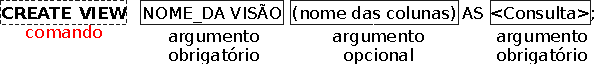
\includegraphics[keepaspectratio,width=\textwidth]{create_view}

\end{frame}

\begin{frame}{Criar visões (views)}

Exemplos:

\begin{alertblock}{OBS: cargo\_id = 1 é o identificador para o cargo de Professor.}
\textbf{CREATE VIEW} professores\_view as SELECT nome, sobrenome, email, cpf, cargo\_id, departamento\_id FROM usuario where cargo\_id = 1;
\end{alertblock}


\pause

\begin{alertblock}{Pode-se depois realizar consultas diretamente na Visão(View)}

\textbf{SELECT} * FROM professores\_view where departamento\_id = 1;

\end{alertblock}

\begin{alertblock}{OBS: departamento\_id=1 é o identificador do DCC.}
\end{alertblock}

\end{frame}

\begin{frame}{Visões Materializadas (Materialised Views)}

Alguns SGBDs permitem que visões sejam armazenadas em disco. Esse tipo de visão é chamada de \textbf{visão materializada (materialised view)}. Caso dados sejam inseridos na base de dados, e o resultado da consulta que define a visão mude, a visão materializada também é atualizada.

\end{frame}

\begin{frame}{Criar Visões Materializadas (Materialised Views)}

\centering 
\includegraphics[keepaspectratio,width=\textwidth]{create_materialised_view}

\end{frame}

\begin{frame}{Criar Visões Materializadas (Materialised Views)}

\begin{alertblock}{}
\textbf{CREATE MATERIALIZED VIEW} professores\_view as SELECT nome, sobrenome, email, cpf, cargo\_id, departamento\_id FROM usuario where cargo\_id = 1;
\end{alertblock}

\begin{alertblock}{}

\textbf{SELECT} * FROM professores\_view where departamento\_id = 1;

\end{alertblock}

\end{frame}

%%%%%%%%%%%%%%%%%%%%%%%%%%%%%%%%%%%%%%%%%%%%%%%%%%%%%%
%%%%%%%%%%%%%%%%%%%%%%%%%%%%%%%%%%%%%%%%%%%%%%%%%%%%%%
\section{}

\begin{frame}[plain,allowframebreaks,noframenumbering]{Bibliografia}

\begin{thebibliography}{Garcia-MolinaEtAl, 2008}

\bibitem[Garcia-MolinaEtAl, 2008]{Garcia-MolinaEtAl2008}

Garcia-Molina, H. and Ullman, J. D. and Widom, J.

\newblock{{\em ``Database Systems: The Complete Book"}. 2nd edition. Prentice Hall, 2008.}

\bibitem[PostgreSQLManual, 2018]{PostgreSQL10_2}

PostgreSQL Development Group.

\newblock{{\em ``PostgreSQL 10.2 Documentation"}. 2018.}

\bibitem[SilberchatzEtAl, 2011]{SilberchatzEtAl2011}

Silberschatz, A. and Korth, H.F. and Sudarshan, S.

\newblock	{{\em ``Database Systems"}. 6th edition. McGrawHill, 2011.}

\end{thebibliography}

\end{frame}

\begin{frame}[plain,noframenumbering]

\begin{center}

\includegraphics[keepaspectratio, width=.8\textwidth]{template/happycat-end}
\end{center}
\end{frame}

\end{document}